%include polycode.fmt 
%format ||-> = "\mapsto"
%format veca = "\vec a"
%format vecb = "\vec b"
%format delay1 ="\sigma_1"
%format delayx ="\sigma_x"
%format delay = "\sigma"
%format Delayx = "\Delta_x"
%format Delay1 = "\Delta_1"
%format mylang = "\lambda^{\rightarrow}_{\Delta}"
%format psin = "\psi. n."
%format < = "\langle"
%format > = "\rangle"
%format *> = ">"
%format <--> = "\leftrightarrow"
%format <- = "\leftarrow"
%format -!> = "\overset{!}{\rightarrow}"
%format \\ = "\lambda"
%format <==> = "\leftrightarrow"
%format <||> = "\langle || \rangle"
%format par = "\langle || \rangle"

\chapter{Background}
In this chapter we will briefly present the background needed to read the bulk of this thesis.
First we will show in what ways programming hardware architectures via a hardware description language is different from programming software.
Furthermore we will discuss general models of hardware and how the constraints they are subject to are modelled, including timing representation. 
While timing representation can take many shapes and forms we limit ourselves to synchronous representations, both in this chapter as in the rest of this thesis, simply because \gls{clash} is a synchronous language.
What a synchronous language is, and it differs from other approaches will be discussed in the section about timing representation.

\section{Hardwarematic \& Softwarematic Computation}
Software languages can exist in two forms: one form describes computations, whereas the other form describes how computations are executed on a specific hardware architecture.
The programming language C for instance was developed as an abstraction of assembly, which is a simplistic form of machine programming.
Other languages such as Lips did not aim to be a mere abstraction of a specific machine, but were able to describe computations themselves. 
These computations could then be mapped to a specific architecture, a result of architecture agnostic languages. 
While C was developed as an abstraction of assembly it could also be used to express computation itself.
Efficient execution however was and is still limited to a specific form of architecture, which makes it hard to map a program written in it to a different form of hardware.

Hardware description languages are inherently different in that they should be able to design the hardware architecture \textit{itself}, and as such can not use the same methods of abstraction as programming languages which target a \textit{specific} architecture, or are architecture agnostic.
Major differences include, but are not limited to, distributed memory models and massively parallel execution.
While in the past decades many languages have been created which do not follow the imperative or procedural paradigm, most languages are still bound to a specific form of hardware architecture.
The Von Neumann architecture is used in personal computers and servers exclusively while also being used often in scientific computing, and as such languages which use a similar underlying model usually are the most natural when execution efficiency is important.

Even though the goal of programming languages and hardware description languages is very different, the general process of both these disciplines is much the same.
What we want to do, in both cases, is  
\begin{inparaenum}[\itshape a\upshape)]
\item indentify the nature of the problem to be solved;
\item organize computations which solve these problems;
\item map the entire composition of these computations to a physical machine capable of executing them.
\end{inparaenum}

For hardware description languages the last step is the most complex.
While the architectures to which programming languages map their compositions of computations hide the time it takes to access memory, as well as hiding the time it takes to execute a computation, we cannot do so in the case of hardware description languages.
When writing software we abstract away from the time it takes to do a computation and assume we will have enough space available for doing our computations.
When describing hardware we do not \textit{want} to abstract away from the time it takes it needs to do a computation, since we need to be sure the sequence of events in a system occur in exactly the order in which we specified them.
The major difference between programming languages and hardware description languages is how \textit{real-world constraints} are handled. 
In the case of programming languages most of these constraints are ignored or considered too troublesome to deal with, while hardware description languages need to consider these constraints as they have significant impact on the results of actual computations.

Many programming languages do not only ignore these constraints, the concept of constraints in general is entirely ignored, leading to languages which can express \textit{any} computation, but of which a subset may not be executable in finite time at all, or may not use a bounded amount of memory.
For hardware description languages this is not completely relevant either; we may consider the hardware we are describing to exist `forever', but at the very least we cannot assume we have an infinite amount of space available to do our computations.
The only way to have infinite space for data is to limit the existence of data to a certain time interval; if all data exists infinitely we must also have infinite space if the hardware is designed to run indefinitely.
So while we may consider infinite time in hardware description languages, we may not create infinite structures. 
We may only describe a finite number of structures and may only schedule the usage of these structures to allow indefinite execution.
To be able to schedule the usage of these resources we must also only allow a limited amount of time \textit{per computation}, as without such an upper bound we still cannot guarantee whether these structures can be scheduled at all.
The last limitation is not needed if we do not allow streaming execution using these computations, but in hardware designs there often is a need for streaming or cyclic execution of computations due to the nature of the problems which are solved using custom hardware designs.

\subsection{Computations in Hardware}
When expressing computations in hardware we do not care solely about the computations themselves, but we also care about whether or not these computations use a bounded amount of space.
We can make an analogy here between the computations expressed in hardware design and the computations expressed in programming language.
When we are dealing with Turing-Complete programming languages we cannot be sure, in the general case at least, whether space is bound to an upper limit, nor whether time is bound to an upper limit.
If we consider Turing-Complete programming languages to able to express \textit{partial} functions, then hardware description languages must be able to only express \textit{total} functions. 
If we cannot determine whether a function is total or partial, then we cannot determine whether the computation this function represents terminates or not, and as such we cannot determine whether the hardware design it describes uses a finite amount of space or time.


\section{The (un)typed $\lambda$-calculus}
From the previous section we can conclude that the essential difference between expressing computations in hardware and software lies in the fact that software generally ignores real-world constraints such as time and space.
In many fields in computer science, such as real-time computing systems, modelling of systems which are subject to real-world constraints is done using formal systems.
When using a formal system it becomes possible to prove certain properties of the system that is being \textit{modelled}.
A formal system is therefor always a more abstract model of reality, where undesirable details are left out.

In this chapter we will discuss a small number of these formal systems, including the (un)typed $\lambda$-calculus and the $\pi$-calculus.
The first describes computations through functions, either restricted by a type-system or not.
The second describes computations through ..................

\subsection{The untyped $\lambda$-calculus}
The untyped $\lambda$-calculus is a formal system which expresses computations via functions.
Functions are used in many languages for their power of abstraction: with merely an identifier and a set of function arguments functionality may be hidden from view.
Not only does the abstraction help with controlling complexity, it also increases code re-use as functions may be used at multiple points in code.
Within the untyped $\lambda$-calculus, without any extension, everything is considered a function.
Church has shown through Church-numerals that numbers can be encoded in terms of function application and abstraction.
Other constructs regular programming languages use, such as if-then-else structures which affect control-flow, can be encoded as well.

All this is possible despite the untyped $\lambda$-calculus only consisting of a few basic operations.
The following three basic operations are defined in the untyped $\lambda$-calculus:
\begin{itemize*}
 \item variable
 \item abstraction
 \item application.
\end{itemize*}
These basic operations are expressed in the following grammar:

\begin{changemargin}{1cm}{0cm}
\begin{expansionno}{text only}
\begin{tabular}{lclr}
e       & $\Coloneqq$ &                 & terms: \\
        & ||     & x                     & (variable) \\
        & ||     & $\lambda$x.e         & (abstraction) \\
        & ||     & e e                   & (application) \\
\end{tabular}
\end{expansionno}
\end{changemargin}

Terms can express \textit{any} computation, as proven through the Church-Turing Thesis and as such can be used as a model for computation in general.
For instance, the identity function is a combination of abstraction and a variable: $\lambda x.x$.
Application to a term $t$ then allows a reduction step: $(\lambda x.x) t$ can be reduced to simply $t$.
A term which allows reduction is called a redex, from reducible expression.

We can imagine terms as representing a tree structure.
For instance, when we take the term $(\lambda x.x) (\lambda y.y)$, which is just the identity function applied to the identity function, we can build a tree-like structure which represents the structure of our abstraction and application:\\
\begin{figure}[h]
\centering
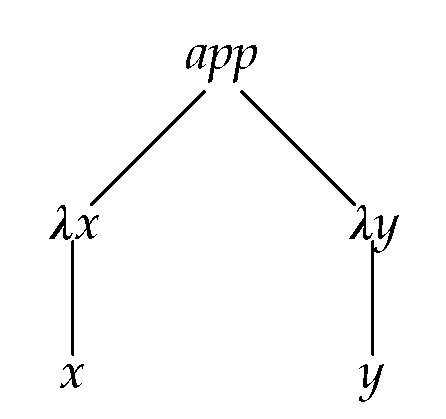
\includegraphics[width=0.2\textwidth]{images/tree}\\
\end{figure}
This structure is called the abstract syntax tree and shows the organisational structure of terms.

The untyped $\lambda$-calculus is a rewriting system. 
Redexes are rewritten by replacing free variables in a term with another term.
For instance, the term $(\lambda x.t_1) t_2$ can be rewritten as $[x \mapsto t_2] t_1$, where $[x \mapsto t_2]$ replaces all free variables in $t_1$ with $t_2$.
A free variable is one which is not bound by any abstraction. 
In the term above, the variable $x$ refers to the binder $\lambda x$.
The term $t_1$ does not contain this exact abstraction, but (may) have a variable which refers to the variable named $x$.

The operation mentioned earlier is called $\beta$-reduction.
Various other reduction strategies exists such as full $\beta$-reduction, normal order reduction, call-by-name and call-by-value and call-by-need which specify the exact conditions under which a reduction can take place.
For a more detailled account see \cite{barendregt1985lambda}.

\subsection{Simply-typed $\lambda$-calculus}
Within the untyped $\lambda$-calculus a number of expressions are considered valid, but when reduced will never reach a normal-form.
A normal form is a state where an expression can no longer be rewritten; the computation is finished.
For instance, the term $\Omega = (\lambda x. x x) (\lambda x. x x)$ will never evaluate to a normal-form.
The term $Y = λf.(λx.f (x x)) (λx.f (x x))$\todo{uitleg}, named the Y-combinator, allows us to define basic recursion.

To disallow these non-normalising functions the simply typed $\lambda$-calculus introduces a type-system, where every term has a well-defined type.
The simply typed $\lambda$-calculus, without a fixpoint-combinator, is strongly normalizing.
Strongly normalizing implies that every valid term will reduce to a normal form without exception.
In practice this is often considered too strict, which is why a fixpoint-combinator is often introduced as a language \textit{primitive}.
A primitive is, like the basic operations of the untyped $\lambda$-calculus, part of the definition of the language.

The simply-typed $\lambda$-calculus is the most simple form of the $\lambda$-calculus which is logically consistent.
Due to this property we can prove termination of programs, and as such it is not turing-complete.\todo{aanname}
Definition \ref{def:lambda} introduces a form of the simply-typed $\lambda$-calculus, $\lambda^\rightarrow$ in short.

\begin{definitiontitled}[text only,float]{Grammar of $\lambda_{\rightarrow}$}{def:lambda}
\begin{changemargin}{-0.5cm}{0cm}
\begin{minipage}[b]{0.50\linewidth}
\begin{tabular}{lclr}
e       & $\Coloneqq$ &                 & expressions: \\
        & ||    & x                     & (variable) \\
        & ||    & $\lambda$x:T.e         & (abstraction) \\
        & ||    & e e                   & (application) \\
        & ||    & c                     & (constant) \\
        & ||    & \textbf{let} x = e \textbf{in} e        & (let binding) \\
\\
c       & $\Coloneqq$ &                 & primitive literals) \\
        & ||    & true                  & (Boolean true) \\
        & ||    & false                 & (Boolean false) \\
        & ||    & n $\in \mathbb{Z}$    & (Integer literals) \\
\end{tabular}
%\captionof{table}{Definition of $\lambda$ with explicit data.}
\end{minipage}
\begin{minipage}[b]{0.40\linewidth}
\begin{tabular}{lclr}
$\tau$  & $\Coloneqq$ &                 & types: \\
        & ||     & $\tau \rightarrow \tau$    & (function type) \\
        & ||     & T                     & (base type) \\
\\
T       & $\Coloneqq$ &                 & base types: \\
        & ||     & Bool                  & (Boolean type) \\
        & ||     & Int                   & (Integer type) \\
\\
$\Gamma$& $\Coloneqq$ &                 & contexts: \\
        & ||     & $\emptyset$           & (empty context) \\
        & ||     & $\Gamma$,x:T          & (term variable binding). \\
\end{tabular}
%\captionof{table}{Definition of $\lambda_{\rightarrow}$}
\end{minipage}
\end{changemargin}
\end{definitiontitled}

This definition shows the addition of a type $\tau$ to the abstraction expression.
Variables which are introduced through $\lambda$-abstraction need to have a type.
This type has one construction operation $\rightarrow$, which constructs a function type from base types.
The base types in this case are Integers and Booleans, but may be expanded in numerous ways.
Polymorphism is not possible in the simply-typed $\lambda$-calculus.
For instance, the general form of the identity function in the untyped $\lambda$-calculus $\lambda x.x$ is not valid in $\lambda^\rightarrow$, as $x$ would need to have a type.
Whenever $x$ has a type, such as in $\lambda x:Int.x$, we can derive the other types.
The $\lambda$-abstraction introduces the $\rightarrow$ construction, which creates the $Int \rightarrow Int$ type, as the result of the identity function has the same type as whatever it is applied to.

That said, the type-system of $\lambda^\rightarrow$ is not complete without typing rules.
Typing rules express the relation between types and terms, and allows us to (partly) infer types of expressions.
We will explain the typing rules of $\lambda^\rightarrow$ next, where we we also explain the meaning of the context $\Gamma$.

\subsubsection{Typing rules}
Typing rules provide the relation between terms and types.
There are three basic approaches to formalizing the semantics of our typing rules:
\begin{itemize*}
\item \textit{Operational Semantics} is a method where the behaviour of rules are defined as a sequence of steps where each step is considered a computation.
\item \textit{Denotational Semantics} uses mathematical constructs such as numbers, sets or functions to give meaning to terms.
\item \textit{Axiomatic Semantics} uses laws to strictly define meaning. This is different from the previous two styles of semantics as there meaning is \textit{derived} from the definition, whereas using axiomatic semantics meaning itself is defined.
\end{itemize*}
Operational semantics is closest to defining an actual implementation, and as such is used to define the typing rules.

We will use $\tau, \sigma, \rho$ to range over types.
The context $\Gamma$ provides the typing environment.
The typing environment is a set of assumptions which must hold.
The assumption $x:\tau$, while introduced informally earlier, states that $x$ has type $\tau$.
Assumptions may be made about the environment as well.
$\Gamma \vdash x : \sigma$ indicates that the context $\Gamma$ provides the type of $x$, and that type is $\sigma$.
The $\vdash$ symbol indicates derivability; we can derive $x : \sigma$ from $\Gamma$.
The above rule is named T-Var and is shown below, together with the other three typing rules of $\lambda^\rightarrow$.
% \begin{changemargin}{1cm}{0cm}

\begin{definitiontitled}[text only]{Typing Rules for $\lambda^\rightarrow$}{def:typerulelambda}
\begin{tabularx}{\textwidth}{ X r X r}
\centering
$ \displaystyle
  \frac
    { x : \sigma \in \Gamma }
    { \Gamma \vdash x : \sigma }
$ & 
T-Var
&
\centering
$ \displaystyle
  \frac
    { c : \sigma \in \Gamma }
    { \Gamma \vdash c : \sigma }
$
&
T-Const
\\
%$ \displaystyle
%  \frac
%    { \Gamma,x:\sigma x \vdash e : \tau }
%    { \Gamma \vdash \lambda x:\sigma.e : \sigma \rightarrow \tau}
%$
\end{tabularx} \\
\\

\begin{tabularx}{\textwidth}{ X r X r}
\centering
$ \displaystyle
  \frac
    { \Gamma,x:\sigma x \vdash e : \tau }
    { \Gamma \vdash \lambda x:\sigma.e : \sigma \rightarrow \tau}
$
&
T-Abs
&
$ \displaystyle
  \frac
    { \Gamma \vdash e_1 : \sigma \rightarrow \tau \quad \Gamma \vdash e_2 : \sigma }
    { \Gamma \vdash e_1 e_2 : \tau }
$
& 
T-App
\\
\end{tabularx}\\
\\

\begin{tabularx}{\textwidth}{X r l X}
 &
$ \displaystyle
  \frac
    { \Gamma \vdash e_1 : \sigma \quad \Gamma,x:\sigma \vdash e_2 : \tau}
    { \Gamma \vdash \textbf{let } x=e_1 \textbf{ in } e_2 : \tau}
$ 
& 
T-Var
&
\\
\end{tabularx}
\end{definitiontitled}

The rule T-Const is trivial as well. 
When the context provides the type $\sigma$ of a constant $c$, then we may derive $c:\sigma$ from the context.

The rule T-Abs shows the relation between abstraction and the function type constructor $\rightarrow$.
Assuming $x$ has type $\sigma$ in the context $\Gamma$ and we can derive from the same $\Gamma$ that $e$ has type $\tau$, then we can derive from the \textit{same} context that $\lambda x:\sigma.e$ has type $\sigma \rightarrow \tau$.
The T-Abs rule can be seen as formalizing the introduction of the $\rightarrow$ type constructor by the $\lambda$-abstraction expression.

The T-App rule can be considered the inverse of the T-Abs rule, as it eliminates the $\rightarrow$ type constructor.
The rule T-App states that, when $e_1$ has a function type of $\sigma \rightarrow \tau$, and $e_2$ has the same type $\tau$, then we may derive from the context $\Gamma$ that $e_2$, when applied to $e_1$, has type $\tau$.

The T-Let rule shows the relation between let bindings and the type-system.
If we can derive $e_1 : \sigma$ from the context and if from the same context including $e_1 : \sigma$ we can derive $e_2 : \tau$, then the lerm $\textbf{let } x = e_1 \textbf{ in } e_2$ has type $\tau$.
As the simply typed $\lambda$-calculus has no polymorphism the use of the let-binding is limited, as we can only reuse expressions with fixed types.
In the next section we will give an introduction to let-polymorphism and constraint based type-checking, where a limited form of polymorphism is allowed.

\subsection{Let-polymorhism and Type Inference}
To allow polymorphism multiple approaches can be used.
The System F approach is more general than let-polymorphism, but also does not allow full type-inference.
For the purposes of this thesis, a simple form of polymorphism is enough to introduce the concept of how polymorphism could be used.
In the next chapter we will introduce a system which is based on the same principle as let-polymorphism, which is another reason for choosing to introduce let-polymorphism.
In this section we will first introduce type variables and how we use them in creating typing constraints.
Afterwards we will introduce unification, which is used to verify whether a set of constraints lead to a well-typed expression.
Using unification as a basis for well-typedness, we can then define type-inference rules, much like the typing rules from before, which define how we may infer princple types from expressions.

\subsubsection{Extending $\lambda^\rightarrow$ with type variables}
As shown in the previous section, let-bindings have the potential to introduce polymorphism.
If we were to define the expression $e = \lambda f.\lambda x. \textbf{let } id = \lambda y.y \textbf{ in } id (f (id x))$, then without defining the type of $x$ and $f$ we could, in principal, derive the type of this expression.
When we introduce a type variable $X$, we can still give an abstract type to $id$. From the definition we know that $\lambda x.x$ only has a single, unknown type involved.
When we call this variable $X$, then the term $id$ would have type $X \rightarrow X$.

Definition \ref{def:lambdaconstraint} extends the grammar of $\lambda^\rightarrow$, to allow type-level variables and ascription.
The majority of the changes have little to do with the grammar however, which is why not much has changed compared to the grammar of $\lambda^\rightarrow$.
The majority of the changes will be explained below, starting with the set of typing constraints.

\begin{definitiontitled}[text only,float]{Grammar of $\lambda_\mathcal{C}^\rightarrow$}{def:lambdaconstraint}
\begin{tabular}{lclr}
$\tau$  & $\Coloneqq$ & $X$             & (type variable) \\
        & ||     & $\ldots$              & \\
\\
$e$     & $\Coloneqq$ & $e$ as T        & (type ascription) \\
        & ||           & \ldots          & \\
\end{tabular}
\end{definitiontitled}

\subsubsection{Constraints}
Using $X \rightarrow X$ as the type of $id$ in the expression $e_1 = id e_2$, we know that the type of $e_1$ must be the same as the type of $e_2$.
These properties are called typing constraints and are defined in definition \ref{def:constraint}.

\begin{definitiontitled}[text only,float]{Set of constraints $\mathcal{C}$}{def:constraint}
Let $\tau$ and $\sigma$ be type expressions as per the grammar of $\lambda_\mathcal{C}$, then the $i^{th}$ \textbf{type-constraint} $\mathcal{C}_i$ is defined as follows as an element of the set $\mathcal{C}$.
\[
\mathcal{C}= \{\mathcal{C}_i || i \in 1..n\} \quad
\mathcal{C}_i = \tau = \sigma
\]
\end{definitiontitled}

Whenever these constraints do not conflict a term is well-typed.
For instance, given a function $f : \textit{Bool} \rightarrow \textit{Int}$, when we use this in $\lambda x:\textit{Bool}. g (f \: x) x$ with $g : X \rightarrow X \rightarrow X$, then $X = \textit{Bool}$ and $X = \textit{Int}$ would conflict, and thus not leading to a well-typed expression.

\subsubsection{Unification}
Unification allows us to systematically find \textit{substitutions} such as $[X \mapsto \textit{Bool}]$ from the previous paragraph.
During the search for substitutions unification also finds conflicts in substitutions and can thus define whether or not a term is well-typed.

The algorithm is fairly straightforward.
Given a set of constraints we can define the following algorithm in pseudo-code:
\begin{changemargin}{1cm}{0cm}
\begin{expansionno}{text only}
\begin{code}
unify = unify 
\end{code}
\end{expansionno}
\end{changemargin}

\subsubsection{Principal Types}
Informally we can define a most general type of an expression, where every unknown type has a unique type variable associated with it.
\citeauthor{pierce2002types} define\cite{pierce2002types} this formally as principal types, which can be referenced if a formal understanding is desired.
For the purposes of this thesis however, this is not needed.
Principal types allow us to define functions \textit{without} type annotations, and where through \textit{type inference} the (principal) types of expressions may be determined.
This principal type can be interpreted as the polymorphic type of an expression.

\begin{definitiontitled}[text only]{Typing Rules for $\lambda^\rightarrow$}{def:typerulelambda}
\begin{tabularx}{\textwidth}{ r r X r}
\centering
$ \displaystyle \frac{ x:\sigma \in \Gamma
}{      \Gamma \vdash x:\sigma ||_{\varnothing} \: \{\}}
$ &
CT-Var
&
$ \displaystyle 
\frac{  \begin{array}{c}
          \Gamma,x:X_1 \vdash e : \tau \: ||_{\mathcal{X}} \: \mathcal{C}\\
          \mathcal{C}' = \mathcal{C} \cup \{ X_2 = X_1 \rightarrow \tau \}  \\
          unique(\mathcal{X},X_1,X_2) \\
        \end{array}
} { \Gamma \vdash \lambda x.e : X_2 \: ||_{X_1 \cup X_2 \cup \mathcal{X}} \: \mathcal{C}'}
$ 
& CT-Abs \\
\\

$ \displaystyle \frac{  \begin{array}{c} 
                          \Gamma \vdash e : X_1 \: ||_{\mathcal{X}} \: \mathcal{C} \\
                          \mathcal{C}' = \mathcal{C} \cup \{ X_1 = \sigma \}
                        \end{array}}
{ \Gamma \vdash (e \text{ as } \sigma) : \sigma \: ||_{\mathcal{X}} \: \mathcal{C}' }
$
& CT-As &
$ \displaystyle
\frac{  \begin{array}{c}
          \Gamma \vdash e_1 : \sigma \: ||_{\mathcal{X}_1} \: \mathcal{C}_1 
            \quad \Gamma \vdash e_2 : \tau \: ||_{\mathcal{X}_2} \: \mathcal{C}_2 \\
          \mathcal{C}' = \mathcal{C}_1 \cup \mathcal{C}_2 \cup \{\sigma = \tau \rightarrow X\} \\
          unique(X,\mathcal{X}_1,\mathcal{X}_2) \\
        \end{array}
} { \Gamma \vdash e_1 \: e_2 : X \: ||_{\mathcal{X}_1 \cup \mathcal{X}_2 \cup X} \: \mathcal{C}' }
$ & CT-App \\
\\

$ \displaystyle
  \frac
    { c : \sigma \in \Gamma }
    { \Gamma \vdash c : \sigma ||_{\varnothing} \{\}}
$
&
CT-Const
& 

$ \displaystyle
  \frac
  { \Gamma \vdash [ x \mapsto e_1] e_2 : \tau \quad \Gamma \vdash e_1 : \sigma }
  { \Gamma \vdash \textbf{let } x = e_1 \textbf{ in } e_2 : \tau} 
$
&
CT-Let
\\
\end{tabularx}

\end{definitiontitled}

\section{Timing representation}
\todo[inline]{Heeft nog wat werk nodig, dit is gewoon c/p van eerder werk}
Aside from the level of abstraction, there are also timing representations to consider. 
For hardware, timing is very important. 
If we view time as continuous, then we can see hardware as a reactive system which continuously reacts to stimuli on the smallest level.
Whenever a certain computation is made in a physical system it will take a certain amount of time for the results of this computation to become stable.
When composing multiple systems or processes then each process will need its inputs stable, leading to a certain delay to start this process. 
What is important to realize is that the resulting implementation has certain timing constraints, but the model on which the physical implementation is based might have an implicit or an explicit notion of time, depending on the criteria of the designer.
\cite{jantsch2005models} and \cite{chang1997heterogeneous} give an excellent overview of the different timing models used within hardware design.
Out of these models we will focus on the synchronous and discrete timing models, since these are the areas that naturally fit in the context of \gls{clash} and this thesis.
We will discuss the following models:
\begin{itemize}
 \item Discrete event models
 \item Synchronous models
 \item Dataflow models
\end{itemize}

These three different timing models have different properties and come more natural to describe certain problems, but will not be suited for all different problem types. 
Within discrete event models entities react to events which occur at a specific time instance and which may only produce values at the same time instance or at a later time instance. 
Execution is chronological in the sense that earlier events are executed before later events.
According to \cite{chang1997heterogeneous}, time is an integral part of the discrete event model, which brings the definitions of discrete event models and discrete time models as mentioned by \cite{jantsch2005models} together.

Discrete event models then describe time by natural numbers where each different moment in time is assigned a value. 
A certain value is valid at a certain point in time, or phrased differently: each event, namely the production of a value, has specific timing information added to it, which gives the total sequence of events a natural ordering. 
Discrete-time models are used in simulation of both \gls{vhdl} and Verilog. 
Within this model combinational logic can both be described as having zero delay, which is easier conceptually, or having a certain non-zero delay which conforms more to a physical circuit. 
The latter is often used for synthesis, where clockspeed of an entire circuit can be derived from the critical path in said circuit. 

Abstracting away from this concept gives synchronous\footnote{Note that synchronous in this context is meant as ``computation having zero delay, not synchronous as in a clocked circuit.''} models, where the moments in time do not denote physical units in time, but represent abstract moment in time. 
Due to this abstraction it is easier for the designer to focus on functionality, as he only needs to make sure the correct values are synchronized as opposed to making sure the values are available at the same time and long enough for the computation to be done.
According to \cite{jantsch2005models} this leads to a clean separation between communication and computation, as each computation is instantaneous and the entire clockcycle is used for communication between processes. 
The assumption that computation is instantaneous is called the \tif{synchrony hypothesis}.
Aside from a clean separation between communication and computation the sychronous model offers easy composition.
In a synchronous model, components can be decomposed and composed without having any real influence on the model used, as mentioned by \cite{benveniste1991synchronous}.
When composing components the actual delay, in the physical sense, that occurs is increased, though in the model itself the entire component still takes one cycle. 
This makes developing hardware possible without dealing with an explicit notion of time.
If cyclic dependencies are allowed in the synchronous language then according to \cite{chang1997heterogeneous} execution of the language involves finding a \textit{fixed point}, or a consistent value for all events at a given time instant.

Dataflow languages have no concept of time, since they only define what should happen given enough tokens are available as inputs.
Communication then takes place in \textit{streams} of values, each containing a various number of tokens.
A data flow language is a language that describes a system in terms of data dependencies between processes. 
\cite{ackerman1982data} mentions there are several properties to keep in mind when discussing data flow, of which I will cite the relevant ones to hardware description:
\begin{itemize}
 \item 
    ``Freedom from side effects.''
    This is a property that works extremely well with functional languages.
    Pure functions are inherently side effect free, so modelling processes as having no side effects is natural to functional languages.
 \item
    ``Locality of effect.''
    Similarly to the previous property, this one works well with functional languages for the same reasons.
 \item 
    ``A "single assignment" convention.''
    Variables can be seen as labeled wires within a hardware design. 
    If viewed as such then the single assignment convention not only makes sense, but should be enforced to not have multiple drivers of a signal.
 \item 
    ``A somewhat unusual notation for iterations, necessitated by freedom from side effects and single assignment.''
    This property does not really work well with functional languages, but highlights a major `shortcoming' of functional languages. Iterations have to be done using recursion, which cannot easily be translated to hardware. This issue will be explored in greater detail later.
 \item
    ``A lack of `history sensitivity' in procedures.'' 
    As the authors already mention, this is not really true in all cases, and this is especially not the case for hardware designs.
\end{itemize}

There are many different languages and models in use today to express dataflow.
One of the commonly used models is SDF\cite{lee1987synchronous}, which allows \textit{static scheduling}, a property which important for being able to construct a schedule from static information.
There are also a various number of languages that are based of the same synchronous principle, such as Lustre\cite{halbwachs1991synchronous}, Signal\cite{amagbegnon1995implementation} and many others.

